\documentclass[spec, och, labwork]{shiza}
% параметр - тип обучения - одно из значений:
%    spec     - специальность
%    bachelor - бакалавриат (по умолчанию)
%    master   - магистратура
% параметр - форма обучения - одно из значений:
%    och   - очное (по умолчанию)
%    zaoch - заочное
% параметр - тип работы - одно из значений:
%    referat    - реферат
%    coursework - курсовая работа (по умолчанию)
%    diploma    - дипломная работа
%    pract      - отчет по практике
% параметр - включение шрифта
%    times    - включение шрифта Times New Roman (если установлен)
%               по умолчанию выключен
\usepackage{subfigure}
\usepackage{tikz,pgfplots}
\pgfplotsset{compat=1.5}
\usepackage{float}

%\usepackage{titlesec}
\setcounter{secnumdepth}{4}
%\titleformat{\paragraph}
%{\normalfont\normalsize}{\theparagraph}{1em}{}
%\titlespacing*{\paragraph}
%{35.5pt}{3.25ex plus 1ex minus .2ex}{1.5ex plus .2ex}

\titleformat{\paragraph}[block]
{\hspace{1.25cm}\normalfont}
{\theparagraph}{1ex}{}
\titlespacing{\paragraph}
{0cm}{2ex plus 1ex minus .2ex}{.4ex plus.2ex}

% --------------------------------------------------------------------------%


\usepackage[T2A]{fontenc}
\usepackage[utf8]{inputenc}
\usepackage{graphicx}
\graphicspath{ {./images/} }
\usepackage{tempora}

\usepackage[sort,compress]{cite}
\usepackage{amsmath}
\usepackage{amssymb}
\usepackage{amsthm}
\usepackage{fancyvrb}
\usepackage{listings}
\usepackage{listingsutf8}
\usepackage{longtable}
\usepackage{array}
\usepackage[english,russian]{babel}

% \usepackage[colorlinks=true]{hyperref}
\usepackage{url}

\usepackage{underscore}
\usepackage{setspace}
\usepackage{indentfirst} 
\usepackage{mathtools}
\usepackage{amsfonts}
\usepackage{enumitem}
\usepackage{tikz}
\usepackage{minted}

\usepackage{booktabs}

\newcommand{\eqdef}{\stackrel {\rm def}{=}}
\newcommand{\specialcell}[2][c]{%
\begin{tabular}[#1]{@{}c@{}}#2\end{tabular}}

\renewcommand\theFancyVerbLine{\small\arabic{FancyVerbLine}}

\newtheorem{lem}{Лемма}

\begin{document}

% Кафедра (в родительном падеже)
\chair{}

% Тема работы
\title{Цифроаналоговый преобразователь}

% Курс
\course{3}

% Группа
\group{331}

% Факультет (в родительном падеже) (по умолчанию "факультета КНиИТ")
\department{факультета КНиИТ}

% Специальность/направление код - наименование
%\napravlenie{09.03.04 "--- Программная инженерия}
%\napravlenie{010500 "--- Математическое обеспечение и администрирование информационных систем}
%\napravlenie{230100 "--- Информатика и вычислительная техника}
%\napravlenie{231000 "--- Программная инженерия}
\napravlenie{100501 "--- Компьютерная безопасность}

% Для студентки. Для работы студента следующая команда не нужна.
% \studenttitle{Студентки}

% Фамилия, имя, отчество в родительном падеже
\author{автор}

% Заведующий кафедрой
% \chtitle{} % степень, звание
% \chname{}

%Научный руководитель (для реферата преподаватель проверяющий работу)
\satitle{аспирант} %должность, степень, звание
\saname{А. А. Мартышкин}

% Руководитель практики от организации (только для практики,
% для остальных типов работ не используется)
% \patitle{к.ф.-м.н.}
% \paname{С.~В.~Миронов}

% Семестр (только для практики, для остальных
% типов работ не используется)
%\term{8}

% Наименование практики (только для практики, для остальных
% типов работ не используется)
%\practtype{преддипломная}

% Продолжительность практики (количество недель) (только для практики,
% для остальных типов работ не используется)
%\duration{4}

% Даты начала и окончания практики (только для практики, для остальных
% типов работ не используется)
%\practStart{30.04.2019}
%\practFinish{27.05.2019}

% Год выполнения отчета
\date{2022}

\maketitle

% Включение нумерации рисунков, формул и таблиц по разделам
% (по умолчанию - нумерация сквозная)
% (допускается оба вида нумерации)
% \secNumbering

%-------------------------------------------------------------------------------------------

\section*{Цель работы:}

Ознакомление с принципом работы и испытание интегрального цифроаналогового
преобразователя.

\subsection*{Задание 1.}

Соберем схему для испытания интегрального цифроаналогового преобразователя.

\begin{figure}[H]
    \centering
    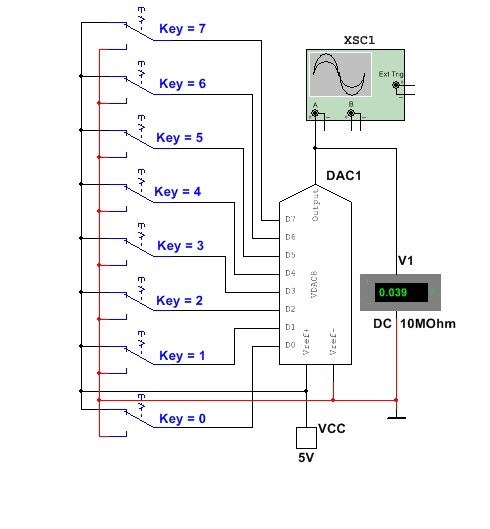
\includegraphics[width=4.58333in,height=5.00833in]{image1.jpeg}
\end{figure}

\subsection*{Задание 2.}

Получим ступенчатое выходное напряжение ЦАП, подавая напряжение 5 В на вход ЦАП
и запустив программу моделирования. На выходе ЦАП формируется напряжение, равное
ЗМР. Затем во время остановок моделирования замыкаем поочередно переключатели 1,
2, \ldots, 7, подавая входные десятичные комбинации 3, 7, \ldots, 255 на входы
D0, \ldots, D7 ЦАП.

\begin{figure}[H]
    \centering
    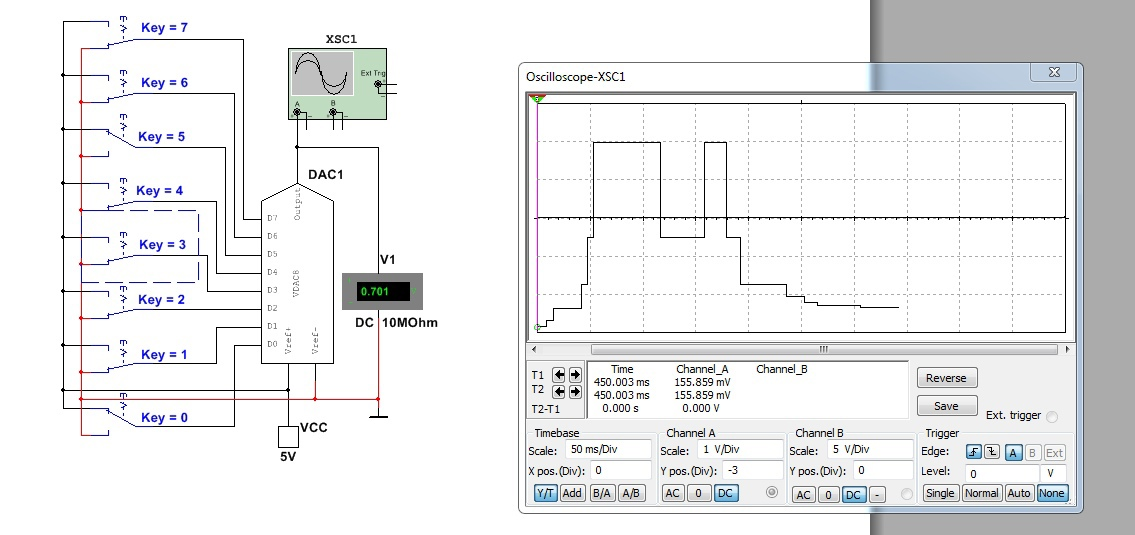
\includegraphics[width=6.49167in,height=3.06667in]{image2.jpeg}
\end{figure}

\begin{table}[H]
    \centering
    \begin{longtable}[]{@{}
    |>{\raggedright\arraybackslash}p{(\columnwidth - 8\tabcolsep) * \real{0.2000}}
    |>{\raggedright\arraybackslash}p{(\columnwidth - 8\tabcolsep) * \real{0.2000}}
    |>{\raggedright\arraybackslash}p{(\columnwidth - 8\tabcolsep) * \real{0.2000}}
    |>{\raggedright\arraybackslash}p{(\columnwidth - 8\tabcolsep) * \real{0.2000}}
    |>{\raggedright\arraybackslash}p{(\columnwidth - 8\tabcolsep) * \real{0.2000}}@{}|}
    \hline
    \begin{minipage}[b]{\linewidth}\raggedright
    N п/п
    \end{minipage} & \begin{minipage}[b]{\linewidth}\raggedright
    Входной десятичный код N
    \end{minipage} & \begin{minipage}[b]{\linewidth}\raggedright
    Выходное напряжение U\textsubscript{вых}, В
    \end{minipage} & \begin{minipage}[b]{\linewidth}\raggedright
    Напряжение ступени U\textsubscript{вых1} -U\textsubscript{вых2}, В
    \end{minipage} & \begin{minipage}[b]{\linewidth}\raggedright
    \vspace{0.1in}
    Значение младшего разряда МЗР= (U\textsubscript{вых1}
    -U\textsubscript{вых2})/16, В
    \end{minipage} \\
    \hline
    \endhead
    1 & 15 & 0.312 & 0,312 & 0,0195 \\ \hline
    2 & 31 & 0.623 & 0,311 & 0,01943 \\ \hline
    3 & 47 & 0.935 & 0,312 & 0,0195 \\ \hline
    4 & 63 & 1.247 & 0,312 & 0,0195 \\ \hline
    5 & 79 & 1.559 & 0,310 & 0,01937 \\ \hline
    6 & 95 & 1.87 & 0,312 & 0,0195 \\ \hline
    7 & 111 & 2.182 & 0,313 & 0,01956 \\ \hline
    8 & 127 & 2.494 & 0,312 & 0,0195 \\ \hline
    9 & 143 & 2.805 & 0,312 & 0,0195 \\ \hline
    10 & 159 & 3.117 & 0,311 & 0,01943 \\ \hline
    11 & 175 & 3.429 & 0,311 & 0,01943 \\ \hline
    12 & 191 & 3.741 & 0,312 & 0,0195 \\ \hline
    13 & 207 & 4.052 & 0,313 & 0,01956 \\ \hline
    14 & 223 & 4.364 & 0,312 & 0,0195 \\ \hline
    15 & 239 & 4.676 & 0,310 & 0,01937 \\ \hline
    16 & 255 & 4.988 & 0,311 & 0,01943 \\ \hline
    \end{longtable}
\end{table}


\subsection*{Задание 3.}

Соберем схему для испытания цифроаналогового преобразователя и установим в
диалоговых окнах компонентов их параметры или режимы работы.

\begin{figure}[H]
    \centering
    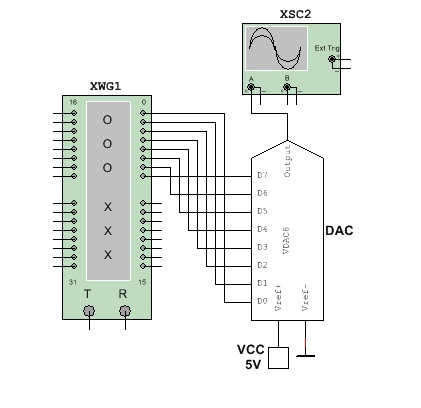
\includegraphics[width=4.38333in,height=4.13333in]{image3.jpeg}\\
\end{figure}

Проведем моделирование ЦПА, запрограммировав генератор на возрастании и убывании
шестнадцатеричных чисел от 0 до FF при шаге 16\textsubscript{10}.

\begin{figure}[H]
    \centering
    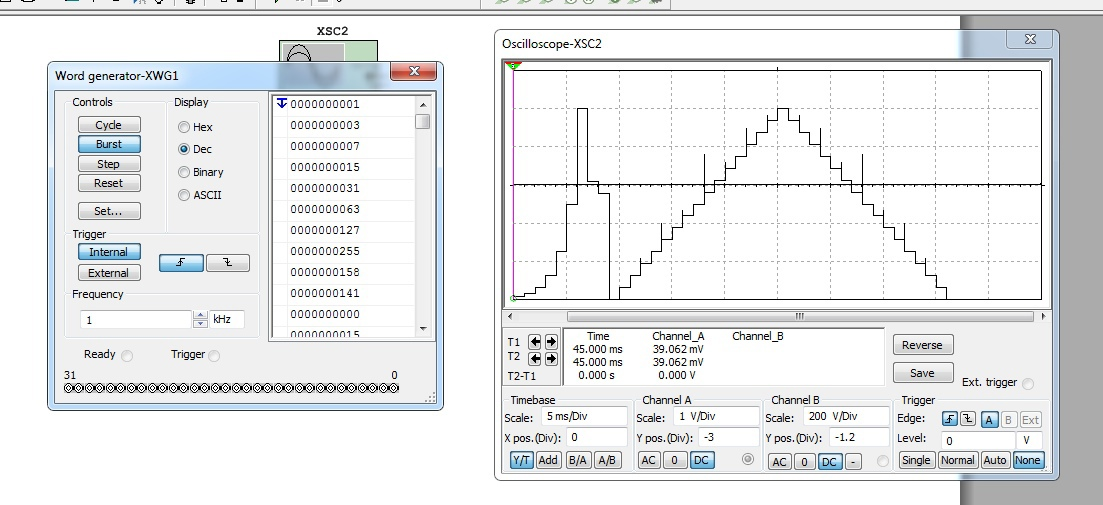
\includegraphics[width=6.49167in,height=2.85in]{image4.jpeg}
\end{figure}

\textbf{Вывод:} ознакомились с принципом работы и испытали интегральный
цифроаналоговый преобразователь.


\section*{Тестовые задания к работе 35}

\begin{enumerate}
    \item 
        \textit{Укажите \textbf{назначение} ЦАП}:

        для преобразования цифрового кода N в пропорциональное аналоговое
        значение напряжения $u(N)$;

    \item
        \textit{Укажите, какая \textbf{структура резистивных матриц} ЦАП имеет
        преимущество при изготовлении преобразователя посредством интегральной
        технологии}:

        матрица R"=2R.

    \item
        \textit{Определите понятие \textbf{<<абсолютная разрешающая
        способность>>} ЦАП}:

        это среднее значение минимального изменения сигнала на выходе ЦАП,
        обусловленное увеличением или уменьшением его кода на единицу.

    \item
        \textit{Укажите, для чего выбирают опорное напряжение
        \textbf{двуполярным}}:

        чтобы получать на выходе двуполярное напряжение $\pm u_\text{вых}$ при
        различных входных кодах;

    \item
        \textit{Укажите \textbf{перспективы развития} ЦАП}:

        \begin{itemize}
            \item повышение быстродействия ключей и уменьшение времени установки ОУ;
            \item применение стабилизированных источников опорного напряжения;
            \item улучшение качества резистивных матриц.
        \end{itemize}
\end{enumerate}

\end{document}
